\documentclass[tikz,border=5pt]{standalone}
\usepackage{amsmath,amssymb}
\usetikzlibrary{chains,positioning}
\begin{document}
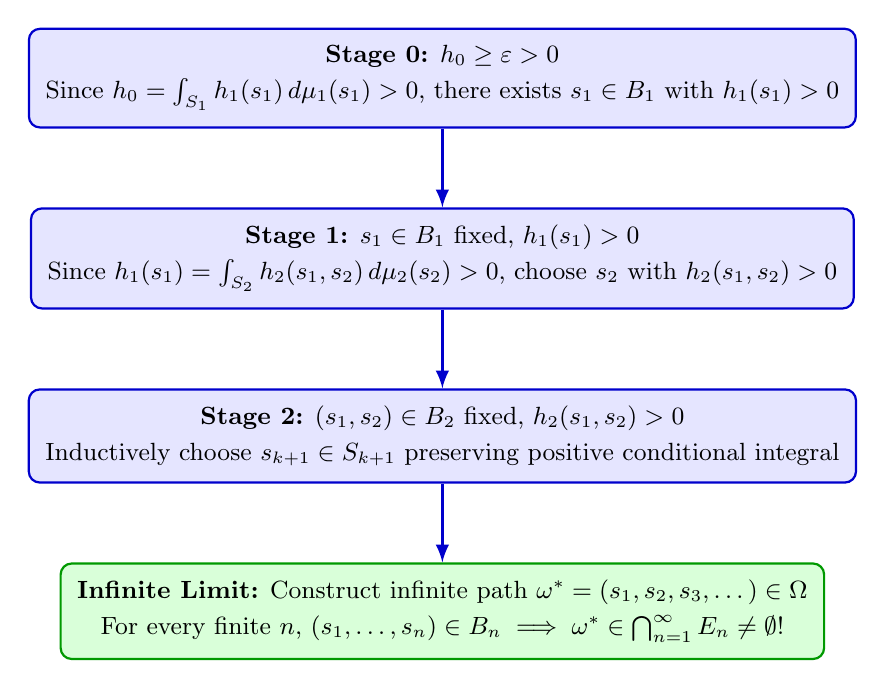
\begin{tikzpicture}[>=latex, font=\small, node distance=1.0cm]
  \node[draw=blue!80!black, fill=blue!10, rounded corners, thick, align=center, inner sep=6pt] (b0)
    {\textbf{Stage 0:} $h_0 \ge \varepsilon > 0$\\[2pt]
     Since $h_0 = \int_{S_1} h_1(s_1)\,d\mu_1(s_1) > 0$, there exists $s_1 \in B_1$ with $h_1(s_1) > 0$};

  \node[draw=blue!80!black, fill=blue!10, rounded corners, thick, align=center, inner sep=6pt, below=of b0] (b1)
    {\textbf{Stage 1:} $s_1 \in B_1$ fixed, $h_1(s_1) > 0$\\[2pt]
     Since $h_1(s_1) = \int_{S_2} h_2(s_1, s_2)\,d\mu_2(s_2) > 0$, choose $s_2$ with $h_2(s_1, s_2) > 0$};

  \node[draw=blue!80!black, fill=blue!10, rounded corners, thick, align=center, inner sep=6pt, below=of b1] (b2)
    {\textbf{Stage 2:} $(s_1, s_2) \in B_2$ fixed, $h_2(s_1, s_2) > 0$\\[2pt]
     Inductively choose $s_{k+1} \in S_{k+1}$ preserving positive conditional integral};

  \node[draw=green!60!black, fill=green!15, rounded corners, thick, align=center, inner sep=6pt, below=of b2] (b3)
    {\textbf{Infinite Limit:} Construct infinite path $\omega^* = (s_1, s_2, s_3, \dots) \in \Omega$\\[2pt]
     For every finite $n$, $(s_1, \dots, s_n) \in B_n \implies \omega^* \in \bigcap_{n=1}^\infty E_n \neq \emptyset$!};

  \draw[->, very thick, blue!80!black] (b0) -- (b1);
  \draw[->, very thick, blue!80!black] (b1) -- (b2);
  \draw[->, very thick, blue!80!black] (b2) -- (b3);
\end{tikzpicture}
\end{document}
